\documentclass[main.tex]{subfiles}
\begin{document}
\begin{enumerate}

\subsection*{Section 4 Electromagnetics, Radiation Systems \& Microwave Engineering}

\item [10.] The magnetic field of a particular mode in a parallel-plate air waveguide with a plate separation of 2.5 cm is given by
$$H_{z}(x, y)=C e^{-j 640 \pi x / 3} \cos (160 \pi y)$$
where x and y are both in meters.
    
    \begin{enumerate}
        \item \textbf{Q.} Is this a TE\textsubscript{n} or TM\textsubscript{n} mode? What is n? Is it a propagating or non-propagating mode? \textbf{Theory.} For Transverse electric (TE) modes there is no electric field in the direction of propagation. These are sometimes called H modes because there is only a magnetic field along the direction of propagation (H is the conventional symbol for magnetic field). For Transverse magnetic (TM) modes there is no magnetic field in the direction of propagation. These are sometimes called E modes because there is only an electric field along the direction of propagation. We will compare the given magnetic-field expression with the one obtained in the textbook after the study of the parallel-plate waveguides. Based on the comparison, we will obtain the mode type, $\bar{\gamma}$ and $a$. \textbf{A.} Consider the propagation direction is $x$ instead of $z$. The general form of a magnetic field for Transverse Magnetic (TM) mode is
        
        $$
        H_z(x, y)=C_1 e^{-\gamma^x} \cos \left(\frac{m \pi}{a}\right) y.
        $$
        
        and by comparing equations it is clear that the given magnetic field expression represents a $\mathrm{TM_n}$ mode of a waveguide  where the guide propagation constant

        $$
        \bar{\gamma} &= \frac{j 640 \pi}{3} \mathrm{rad}/\mathrm{m}
        $$

        and

        $$
        \frac{m \pi}{a} &= 160 \pi.
        $$
        
        Here $a=2.5 \mathrm{~cm}=2.5 \times 10^{-2} \mathrm{m}$

        $$
        \begin{aligned}
        \frac{m \pi}{2.5 \times 10^{-2}} &= 160 \pi \\
        m &= 4
        \end{aligned}
        $$

        Therefore, it is $\mathrm{TM_4}$ mode. The constant $\gamma$ is purely imaginary therefore it is a propagating mode.
        
        \item \textbf{Q.} What is the operating frequency? \textbf{Theory.} To obtain $f$, we need to obtain the cut off frequency $f_{c m}$ using
        
        $$
        f_{cm}=\frac{mc}{2 a}
        $$
        
        Next, we will solve the following equation for $f$ :
        $$
        \bar{\gamma}_m=j \beta \sqrt{1-\left(\frac{f_{c m}}{f}\right)^2}=\frac{j 2 \pi f}{c} \sqrt{1-\left(\frac{f_{c m}}{f}\right)^2}
        $$
        
        \textbf{A.} The cutoff frequency of the $\mathrm{TM}_4$ mode is
        
        $$
        \begin{aligned}
        f_{c 4} & =\frac{m c}{2 a} \\
        & =\frac{4\left(3 \times 10^8\right)}{2\left(2.5 \times 10^{-2}\right)} \\
        & =24 \mathrm{GHz}
        \end{aligned}
        $$

        Because the $\mathrm{TM}_4$ mode is a propagating mode, the mode propagation constant is given by
        
        $$
        \begin{aligned}
        \bar{\gamma}_4 & =j \beta \sqrt{1-\left(\frac{f_{c m}}{f}\right)^2} \\
        & =j \frac{2 \pi f}{c} \sqrt{1-\left(\frac{f_{c 4}}{f}\right)^2} \\
        & =j \frac{2 \pi}{c} \sqrt{f^2-f_{c 4}^2}
        \end{aligned}
        $$

        Substituting $\bar{\gamma}_4=\frac{j 640 \pi}{3}$ and $f_{c 4}=24 \mathrm{GHz}$ gives
        
        $$
        \frac{j 640 \pi}{3}=\frac{j 2 \pi}{3 \times 10^8} \sqrt{f^2-\left(24 \times 10^9\right)^2}
        $$
        
        or
        
        $$
        f^2-\left(24 \times 10^9\right)^2=\left(32 \times 10^9\right)^2
        $$
        
        Thus,
        
        $$
        f=40 \mathrm{GHz}
        $$
        
        \item \textbf{Q.} Find the corresponding electric field. \textbf{Theory.} To obtain the electric field we will use the following relations:
        
        $$
        \begin{gathered}
        \mathbf{E}=E_x \hat{\mathbf{x}}+E_y \hat{\mathbf{y}} \\
        E_x=\frac{1}{j \omega \epsilon_0} \frac{\partial H_z}{\partial y} \text { and } E_y=-\frac{1}{j \omega \epsilon_0} \frac{\partial H_z}{\partial x}
        \end{gathered}
        $$ 
        
        \textbf{A.} For a TM mode of a waveguide that is infinite in extent in the $x$ and $z$ directions and waves are guided in $x$ direction, we have
        
        $$
        H_x=0 ; E_x \neq 0
        $$
        
        and
        
        $$
        \begin{gathered}
        \mathbf{E}=E_x \hat{\mathbf{x}}+E_y \hat{\mathbf{y}} \\
        \mathbf{H}=H_z \hat{\mathbf{z}}
        \end{gathered}
        $$
        
        It is given that
        
        $$
        H_z(x, y)=C_1 e^{-j 640 \pi x / 3} \cos (160 \pi y)
        $$

        We can obtain $E_x$ as
        
        $$
        \begin{aligned}
        E_x & =\frac{1}{j \omega \epsilon_0} \frac{\partial H_z}{\partial y} \\
        & =\frac{1}{j \omega \epsilon_0} \frac{\partial}{\partial y}\left[C_1 e^{-j 640 \pi x / 3} \cos (160 \pi y)\right] \\
        & =\frac{C_1 e^{-j 640 \pi x / 3}}{j \omega \epsilon_0} \frac{\partial}{\partial y}[\cos (160 \pi y)] \\
        & =-\frac{160 \pi C_1 e^{-j 640 \pi x / 3}}{j 2 \pi f \epsilon_0} \sin (160 \pi y) \\
        & =-\frac{160 \pi}{j 2 \pi f \epsilon_0} C_1 \sin (160 \pi y) e^{-j 640 \pi x / 3} \\
        & =\frac{j 160 \pi}{2 \pi \epsilon_0\left(40 \times 10^9\right)} C_1 \sin (160 \pi y) e^{-j 640 \pi x / 3} \\
        & =j 225.9 C_1 \sin (160 \pi y) e^{-j 640 \pi x / 3}
        \end{aligned}
        $$

        We find $E_y$ as follows:
        
        $$
        \begin{aligned}
        E_y & =-\frac{1}{j \omega \epsilon_0} \frac{\partial H_z}{\partial x} \\
        & =-\frac{1}{j \omega \epsilon_0} \frac{\partial}{\partial x}\left[C_1 e^{-j 640 \pi x / 3} \cos (160 \pi y)\right] \\
        & =-\frac{C_1}{j 2 \pi f \epsilon_0} \cos (160 \pi y) \frac{\partial}{\partial x}\left[e^{-j 640 \pi x / 3}\right] \\
        & =-\frac{C_1}{j 2 \pi f \epsilon_0} \cos (160 \pi y)\left[\frac{-j 640 \pi}{3} e^{-j 640 \pi x / 3}\right] \\
        & =-\frac{-j 640 \pi}{j 2 \pi \epsilon_0\left(40 \times 10^9\right)} \cos (160 \pi y) e^{-j 640 \pi x / 3} \\
        & =301.2 C_1 \cos (160 \pi y) e^{-j 640 \pi x / 3}
        \end{aligned}
        $$

        We can express the total electric field as
        
        $$
        \begin{aligned}
        \mathbf{E} & =E_x \hat{\mathbf{x}}+E_y \hat{\mathbf{y}} \\
        & =C_1 e^{-j 640 \pi x / 3}[j 225.9 \sin (160 \pi y) \hat{\mathbf{x}}+301.2 \cos (160 \pi y) \hat{\mathbf{y}}]
        \end{aligned}
        $$
        
    \end{enumerate}
    
\item [11.] An electromagnetic field in free space, $\mu_{0}=4 \pi \times 10^{-7}$ henry/meter, $\varepsilon_0 = 8.85 \times 10^{-12}$ farads/meter, is specified as by the vector phasor 

$$\underline{E}(\underline{r})=\underline{E}_{0} \varepsilon^{-j \underline{k} \underline{g} \underline{r}}$$

where $\underline{E}_{0}=\hat{x}$ the unit vector in the x direction of a rectangular coordinate system (x,y,z).

$$\begin{aligned}
&\underline{r}=x \hat{x}+y \hat{y}+z \hat{z} \\
&\underline{k}=-j \hat{y}+2 \hat{z}
\end{aligned}$$

    \begin{enumerate}
        \item What is the frequency f of the electromagnetic field (Hz)?
        \item Describe the equi-phase surfaces of the field. Write a general equation for the equi-phase surfaces.
        \item Describe the constant magnitude-of-field surfaces. Write a general equation for these equal-magnitude surfaces.
        \item Evaluate the average power as a function of position.
    \end{enumerate}

\item [12.] A plane wave is incident in the interface between two dielectrics $\varepsilon_1$ and $\varepsilon_2$, $\varepsilon_1 > \varepsilon_2$ as shown in figure \ref{fig:12q_a}.

\begin{figure}
\centering\fbox{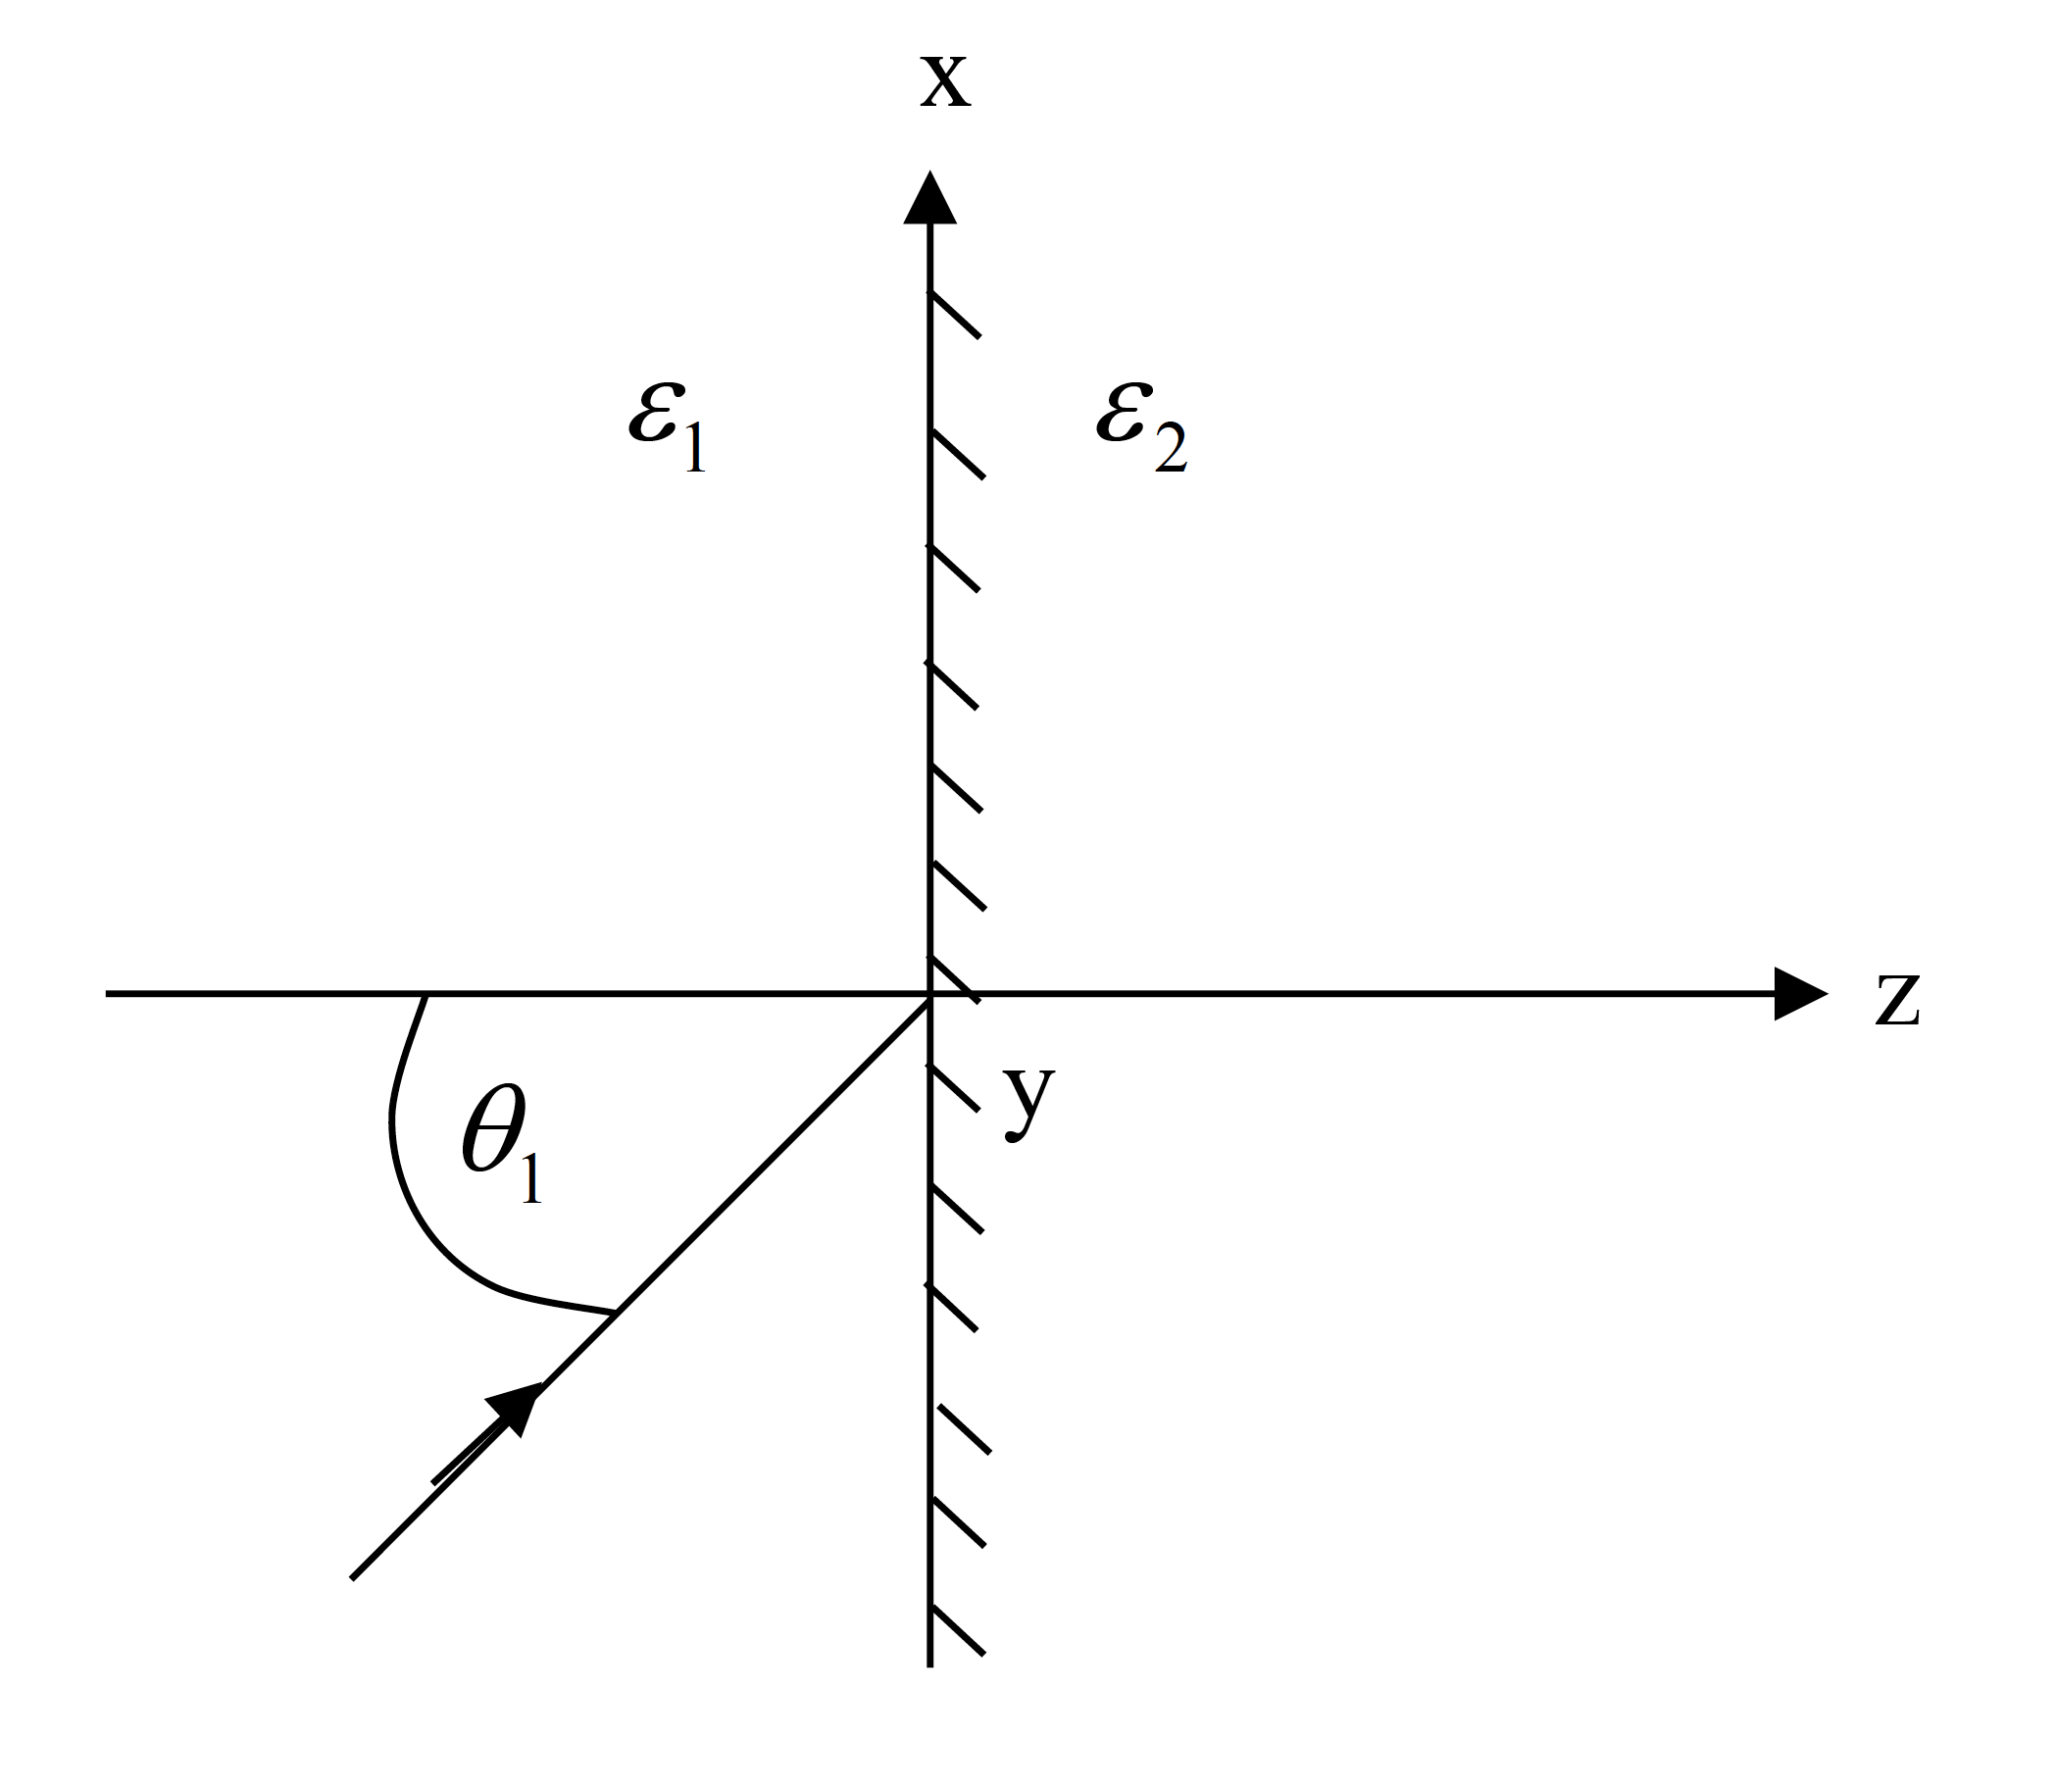
\includegraphics[width=2.0in]{figures/2018s/12q_a.png}}
\caption{Plane wave incident incident in the interface between two dielectrics}
\label{fig:12q_a}
\end{figure}

    \begin{enumerate}
        \item Find the angle $\theta_{1c}$ such that all waves incident with $\theta_1 > \theta_{1c}$ are "totally reflected".
        \item For $\theta_1 > \theta_{1c}$, describe the field (if any) in the region $z > 0$ in the $\varepsilon_2$ dielectric.
        \item If \underline{$E$} is perpendicular to the plane of the incidence, $\underline{E} = E_y \hat{y}$, find the phase of the reflection coefficient.
    \end{enumerate}

\end{enumerate}
\end{document}